
\documentclass{standalone}
\usepackage{xcolor}
\usepackage{pgfplots}
\pgfplotsset{compat=1.18}

\begin{document}

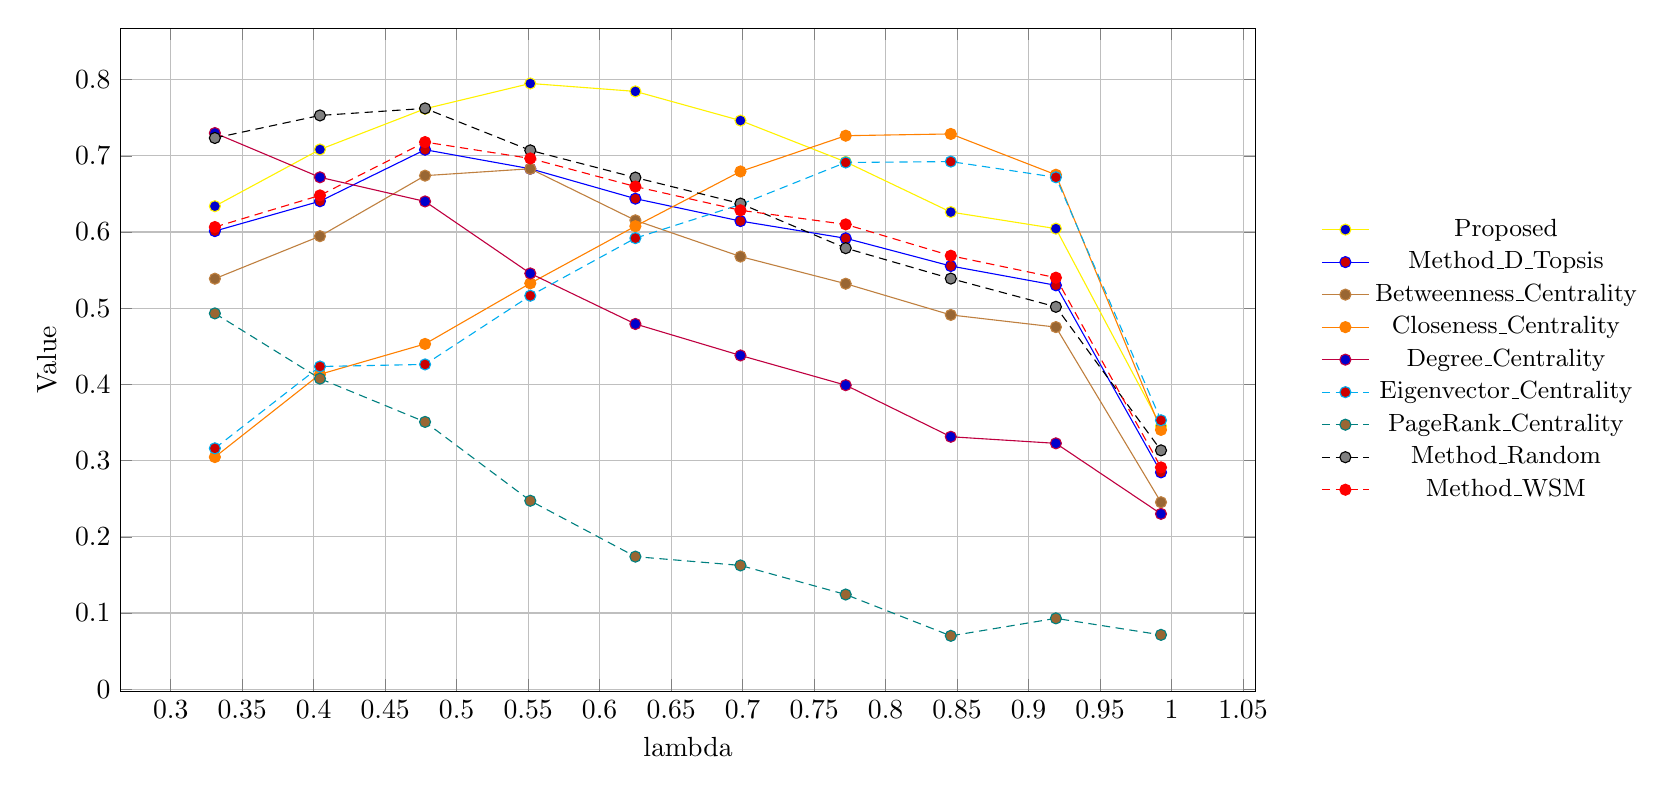
\begin{tikzpicture}
\begin{axis}[
    width=16cm,
    height=10cm,
    xlabel={lambda},
    ylabel={Value},
    grid=major,
    legend style={
        at={(1.05,0.5)},
        anchor=west,
        font=\small,
        draw=none,
        cells={align=left},
    },
]
% Proposed
\addplot+[color=yellow, mark=*] coordinates {
(0.3309,0.6339414300941764) (0.4044,0.7083775668647048) (0.4779,0.761780181322087) (0.5515,0.795000309472499) (0.625,0.7845907134319173) (0.6985,0.7463257230127166) (0.7721,0.6920590929296301) (0.8456,0.6262121657361152) (0.9191,0.6044666470761092) (0.9926,0.3452034343372417) };
\addlegendentry{Proposed}

% Method\_D\_Topsis
\addplot+[color=blue, mark=*] coordinates {
(0.3309,0.6012413455704727) (0.4044,0.6404364424949509) (0.4779,0.7080328012735243) (0.5515,0.6830560945497525) (0.625,0.6438033837976398) (0.6985,0.6143888671310774) (0.7721,0.5917856681228458) (0.8456,0.5553760849069276) (0.9191,0.530078233581718) (0.9926,0.2845780215980019) };
\addlegendentry{Method\_D\_Topsis}

% Betweenness\_Centrality
\addplot+[color=brown, mark=*] coordinates {
(0.3309,0.5387575929456961) (0.4044,0.594557619986399) (0.4779,0.6740134107470781) (0.5515,0.6830517900876585) (0.625,0.615362754556127) (0.6985,0.5678001981724166) (0.7721,0.5321843006890797) (0.8456,0.4911916242850954) (0.9191,0.4752278964958298) (0.9926,0.2453425676502081) };
\addlegendentry{Betweenness\_Centrality}

% Closeness\_Centrality
\addplot+[color=orange, mark=*] coordinates {
(0.3309,0.3046501931768627) (0.4044,0.4132646663754257) (0.4779,0.4531251772226007) (0.5515,0.5326855354618312) (0.625,0.607684440241209) (0.6985,0.6795176279844288) (0.7721,0.7264429054639787) (0.8456,0.7287442527794713) (0.9191,0.6751990553608747) (0.9926,0.3403064378708121) };
\addlegendentry{Closeness\_Centrality}

% Degree\_Centrality
\addplot+[color=purple, mark=*] coordinates {
(0.3309,0.7298995006663058) (0.4044,0.6718152760052861) (0.4779,0.6401590334521037) (0.5515,0.5456927061751112) (0.625,0.4793028384816887) (0.6985,0.4380264200081834) (0.7721,0.3989972428902563) (0.8456,0.3313041683351312) (0.9191,0.3226614509003017) (0.9926,0.2300905573728527) };
\addlegendentry{Degree\_Centrality}

% Eigenvector\_Centrality
\addplot+[color=cyan, mark=*] coordinates {
(0.3309,0.3161165837535475) (0.4044,0.4235191752716265) (0.4779,0.4262345672945529) (0.5515,0.5164139611380456) (0.625,0.5919929605930744) (0.6985,0.6361631852190562) (0.7721,0.691299875001215) (0.8456,0.6924551397621334) (0.9191,0.6718638654276604) (0.9926,0.3529238818575634) };
\addlegendentry{Eigenvector\_Centrality}

% PageRank\_Centrality
\addplot+[color=teal, mark=*] coordinates {
(0.3309,0.493212709105675) (0.4044,0.4076040496873065) (0.4779,0.3507739523378409) (0.5515,0.2473134135438759) (0.625,0.1739770461016941) (0.6985,0.1624246430346526) (0.7721,0.1242455482327567) (0.8456,0.070010332737208) (0.9191,0.0929548955670493) (0.9926,0.0712918025121288) };
\addlegendentry{PageRank\_Centrality}

% Method\_Random
\addplot+[color=black, mark=*] coordinates {
(0.3309,0.7234376720634407) (0.4044,0.753021219776622) (0.4779,0.762270118273661) (0.5515,0.7071985944433212) (0.625,0.671474859827351) (0.6985,0.637340175385974) (0.7721,0.5788311559848334) (0.8456,0.5389030654393493) (0.9191,0.501838771637298) (0.9926,0.3134482556731615) };
\addlegendentry{Method\_Random}

% Method\_WSM
\addplot+[color=red, mark=*] coordinates {
(0.3309,0.6065542293310365) (0.4044,0.648099280739253) (0.4779,0.7180549141974626) (0.5515,0.6965994481485838) (0.625,0.6596997636444951) (0.6985,0.6285127491340907) (0.7721,0.6100397534082272) (0.8456,0.5689074937552956) (0.9191,0.5400797096870334) (0.9926,0.29105909455365) };
\addlegendentry{Method\_WSM}


\end{axis}
\end{tikzpicture}

\end{document}
